% !Mode:: "TeX:UTF-8"
% !TEX program  = xelatex
\section{Introduction}
% 研究的目的、背景;理论依据、实验基础和研究方法或实验设计;预期结果和意义等
\subsection{Dense Prediction Tasks} 
With the rapid development of computer science research and related industries in recent years, people's production and lifestyle have undergone tremendous changes. Breakthroughs have been made in artificial intelligence, especially in the field of machine learning, and it has also been applied in more and more fields.

Neural networks have made impressive results in a variance of tasks \cite{multivandenhende2021}, such as semantic segmentation \cite{long2015fully}, instance segmentation \cite{he2017mask}, augmented reality \cite{abu2018augmented} and panoptic segmentation \cite{kirillov2019panoptic}. All of them are part of a dense prediction task, a collection of computer vision tasks aiming at labeling every pixel in the given image into a predefined class \cite{huang2021fapn}.


\begin{figure}[htb]
    \centering
    \begin{subfigure}[t]{.45\linewidth}
        \centering
        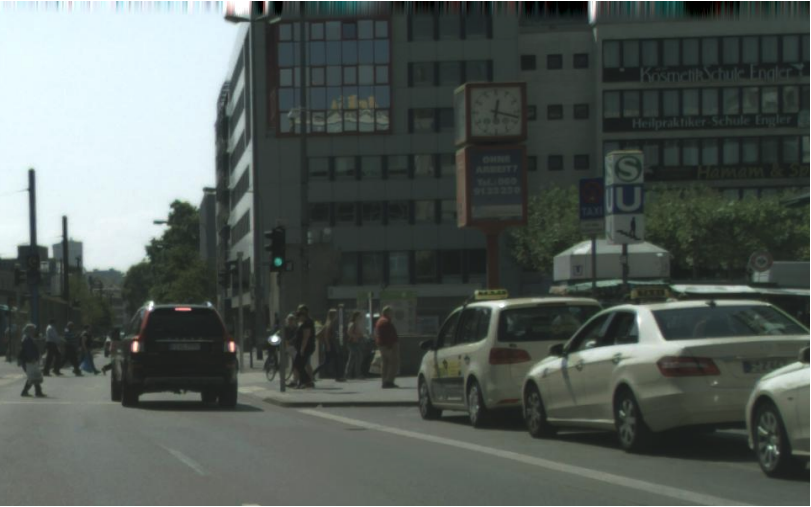
\includegraphics[width=1\textwidth]{figures/RawImage.png}
        \caption{Raw Image}\label{Raw Image}
    \end{subfigure}
    \begin{subfigure}[t]{.45\linewidth}
        \centering
        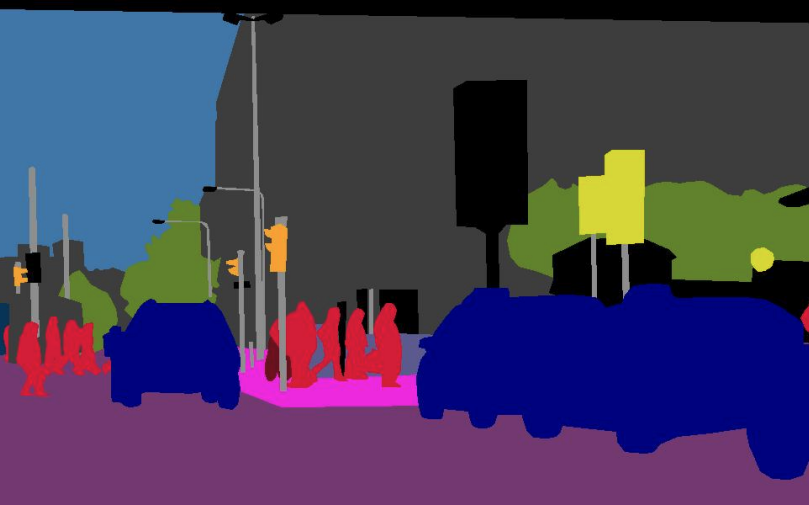
\includegraphics[width=1\textwidth]{figures/Semantic Segmentation2.png}
        \caption{Semantic Segmentation}\label{Semantic Segmentation}
    \end{subfigure}
    \begin{subfigure}[t]{.45\linewidth}
        \centering
        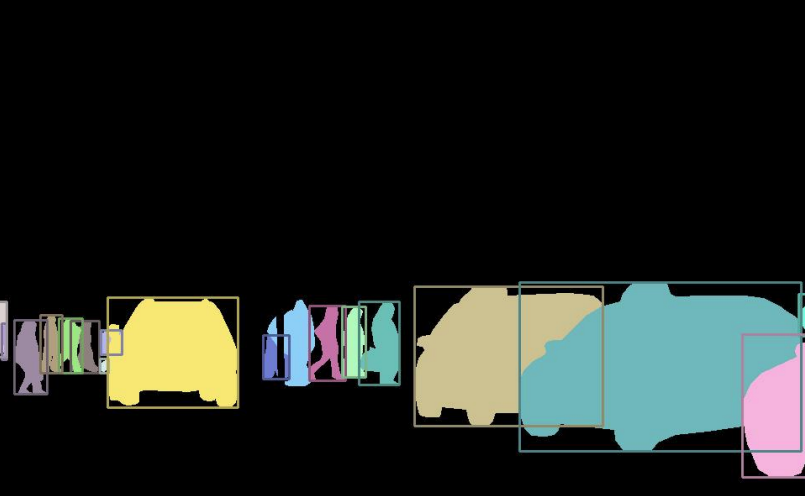
\includegraphics[width=1\textwidth]{figures/Instance Segmentation2.png}
        \caption{Instance Segmentation}\label{Instance Segmentation}
    \end{subfigure}
    \begin{subfigure}[t]{.45\linewidth}
        \centering
        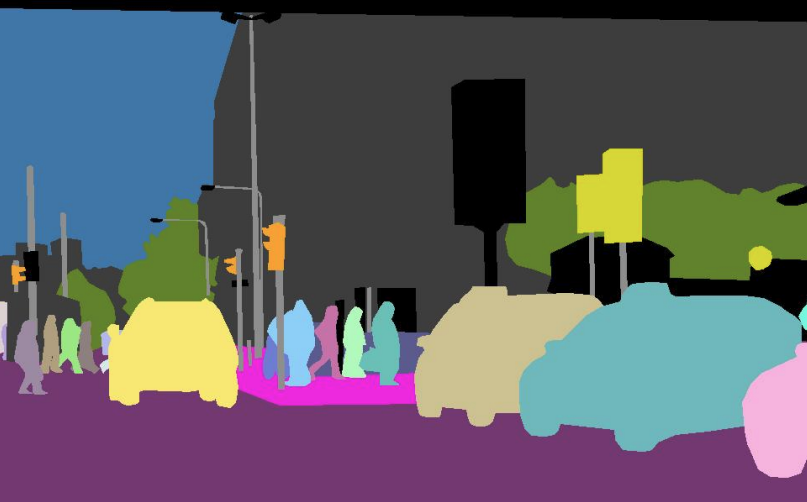
\includegraphics[width=1\textwidth]{figures/PanopticSegmentation.png}
        \caption{Panoptic Segmentation}\label{Panoptic Segmentation}
    \end{subfigure}
    \caption{Computer vision tasks \cite{kirillov2019panoptic}: For a given a) raw image, b) Semantic Segmentation, c) Instance Segmentation, d) Panoptic Segmentation are a part of a dense prediction task, aiming at labeling every pixel in the given image into a predefined class. Panoptic segmentation was proposed by Alexander Kirillov et al. in 2018.}\label{Dense Prediction Tasks}
\end{figure}


Any of these tasks is one of the basic problems of computer vision and has a very high value of use, so it has high importance in various applications, such as autonomous driving \cite{de2017semantic}, medical image segmentation \cite{lei2020medical}, and geospatial object segmentation \cite{zheng2020foreground}.

% Dense prediction可以被视作图像分类任务和目标检测任务的综合任务,其同时需要图像中物体的语义信息和位置信息。为了同时获取两类信息并进行对齐,大多数网络采取了top-down feature pyramid的网络架构。这类网络架构可以获取给定图像不同层级的语义信息;底层网络得到的图像分辨率较高,主要用来获取instance的位置信息;高层图像得到的图像分辨率较低,包含更多抽象的语义信息,用以预测小物体和判断物体边缘的位置。
Dense prediction can be regarded as a comprehensive task of image classification task and object detection task, it needs both semantic information and position information of instances in the given images. To obtain two kinds of information and align them at the same time, most networks adopt the network architecture of the top-down feature pyramid. This type of network architecture can obtain semantic information at different levels of a given image; the image obtained by the lower-level convolution layers has a higher resolution and is mainly used to obtain the location information of the instance; the image obtained by the high-level image has a lower resolution and contains more abstract semantics information for predicting small objects and judging the location of object edges.


\subsection{Apply Dense Prediction on Mobile Terminal} 

Despite all the success mentioned above, most works mainly focuses on applications on server clusters that need powerful computational resources, beyond the capabilities of the mobile terminal, such as mobile phones and embedded devices \cite{zhang2022topformer}. However, in the past few years, the resolution and imaging capabilities of mobile terminal cameras have been significantly improved, meanwhile, mobile computing ability and network bandwidth both have met the requirements for real-time processing of semantic segmentation functions. Most advanced mobile chips have already equipped with a built-in AI chip that can achieve AI computing power exceeding 7 trillion operations per second \cite{qualcommdoc}. Based on the real test scenery of CNN measurement, the actual data of the iPhone XS equipped with Apple A12 is about 5 TOPS \cite{apple}. Makes it possible to deploy and apply the dense prediction method on the mobile terminal. 


\begin{figure}[htb]
    \centering
    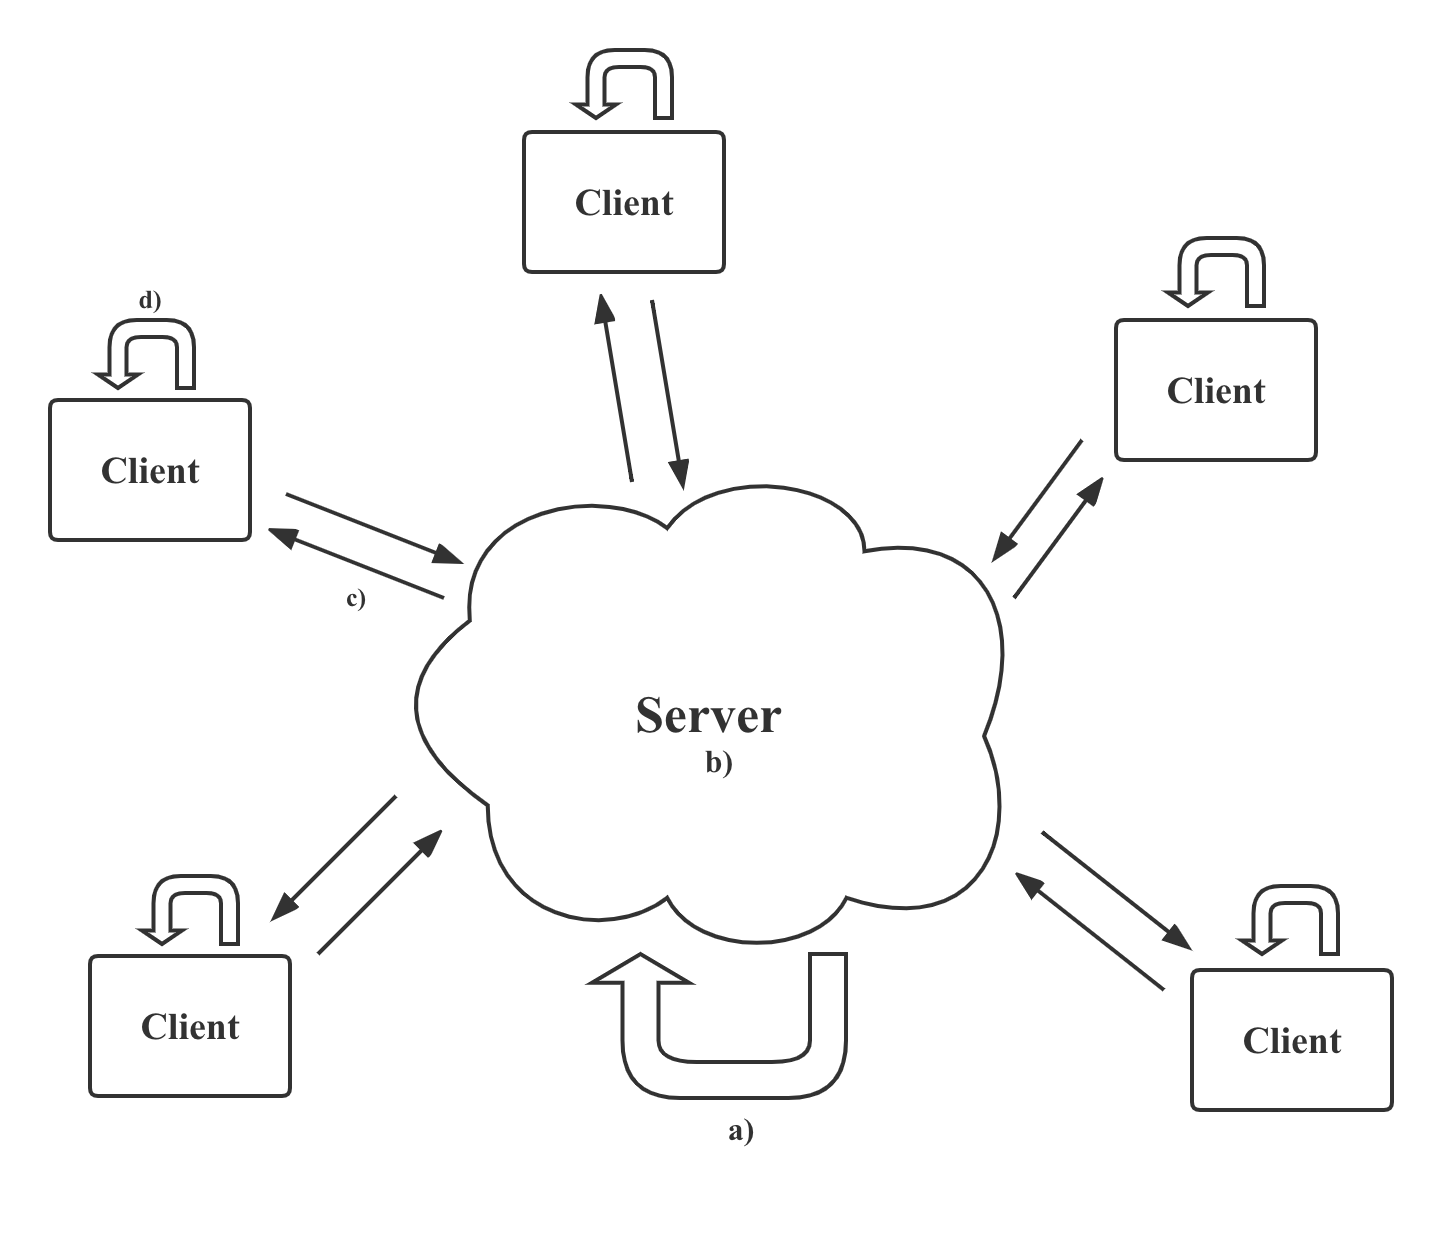
\includegraphics[width=1\textwidth]{figures/ServerClientModule.png}
    \caption{Whole Process Structure: a) Train the specified model. b) Deploy the model on the server. c) Perform the data transmitting. d) Data preprocessing, display and application of mobile segmentation models and other related tasks.}\label{ServerClientModule}
    % 图片的标题应该在下方
\end{figure}

% (移动端计算力和网络带宽/延时均有了显著提升(数据),使得在移动端部署并应用dense prediction方法成为了可能. )
And even to achieve real-time target detection on mobile terminals. The current mainstream mobile operating systems include Apple's IOS system and Android system, among which a huge amount of hardware is equipped with the Android system, which makes it have a huge user group. All mentioned above make it valuable to develop an APP with a dense prediction function on the Android end terminal.

Some traditional image segmentation algorithms such as threshold-based segmentation method \cite{al2010image}, watershed algorithm, and segmentation method based on edge detection, mostly rely on the low-level semantic information of the image to segment the image. Therefore, the segmentation results are not ideal in scenes with complex images and shredded edges. However, the paper FCN (Fully Convolutional Networks for Semantic Segmentation) \cite{long2015fully}, which was a candidate for the best paper in CVPR 2015, has greatly improved the effect of semantic segmentation using pure neural networks. FCN converts the output from a column of feature vectors to a mapped image by replacing traditional CNN's last fully connected layer with a convolutional layer. Thus, the category to which each pixel belongs is recovered from the abstract features, that is, extends from image-level classification to pixel-level classification. FCN laid the foundation for many subsequent semantic segmentation models, including FaPN \cite{huang2021fapn}, ResNet \cite{he2016deep}, etc. used in the paper.


\subsection{Research Objectives and Expected Results}
The goal of the graduation project is to reproduce the training process and results of FaPN \cite{huang2021fapn} and apply this high-accuracy dense prediction model on the mobile terminal, to realize the function of the segment and recognize objects in daily life, such as traffic signs, pedestrian, etc.

In this paper, two methods are applied and deployed on a mobile terminal to obtain better dense prediction results on the mobile terminal. The first kind uses the picture on the mobile terminal through the photo album or camera API, the verified image is then transmitted to the server end for image processing and then re-transmitted back to the front end. Another method is to apply the lightweight paddle-lite \cite{paddlelite} that has been transplanted to the mobile terminal and use the computing power of the mobile phone AI chip to process the image.

The work of paper can be mainly divided into several parts, including deploying and training the model with and without FaPN and evaluating the difference in the model accuracy, loss, AP, and mIoU to reflect the superiority of FaPN. Design an Android APP that allows users to take pictures or use existing images to identify or classify objects. Handle the interaction between the APP front-end and the server back-end. The rest of this thesis is organized as follows. 

Section \uppercase\expandafter{\romannumeral2} \textbf{Related Work}, meanly focus on introducing the main principles and functions of the related modules used and reproduced in this article. This paper gradually understands the structure and innovation of FCN, FPN, FaPN, reproduces the FSM and FAM modules of FaPN, and applies the pre-trained mobile Paddle Lite model.
%介绍本文所用到和复现的相关模块的主要原理和主要功能 本文逐渐深入地了解了FCN,FPN,FaPN的结构和创新点并复现了FaPN的FSM和FAM模块,并应用了预训练的移动端Paddle Lite模型

%主要介绍了APP服务端和客户端的开发过程和对应模块的联系和内容。包括了服务器端的模型的训练和部署,客户端网络,UI等模块的具体功能和结构。
Section \uppercase\expandafter{\romannumeral3} \textbf{FaPN Based APP}, mainly introduces the development process of the APP server and the client and the connection and content of the corresponding modules. It includes the training and deployment of the server-side module, the specific functions and structures of the client-side network, UI, and other modules. 

Section \uppercase\expandafter{\romannumeral4} \textbf{APP Results, Analysis, and Relevant Information}, analyzed training procedure and APP results. Provides information about training and running environments.


Section \uppercase\expandafter{\romannumeral4} \textbf{Conclusion and Future Work}, summarizes existing work and suggests directions for improvement.
\clearpage